\documentclass{article}

% packages
\usepackage{amsmath, amsthm, thmtools, amsfonts, amssymb, luacode, catchfile, tikzducks, hyperref, ifthen}
\ifcsname c@kobocompile\endcsname
	\usepackage[a5paper, total={1072pt, 1448pt}, margin=10pt, includeheadfoot]{geometry} % set page margins
\else
	\usepackage[a4paper, margin=50pt, includeheadfoot]{geometry}
\fi
\usepackage[shortlabels]{enumitem}
\usepackage[skip=3pt, indent=0pt]{parskip}

% language
\usepackage[bidi=basic, layout=tabular, provide=*]{babel}
\ifcsname c@english\endcsname
	\babelprovide[main, import]{english}
\else
	\babelprovide[main, import]{hebrew}
	\babelprovide{rl}
\fi
%\babelfont{rm}{Libertinus Serif}
\babelfont{rm}[Renderer=Harfbuzz]{Libertinus Serif}
\babelfont{sf}{Libertinus Sans}
\babelfont{tt}{Libertinus Mono}

% style
\AddToHook{cmd/section/before}{\clearpage}	% Add line break before section
\linespread{1.3}
\setcounter{secnumdepth}{0}		% Remove default number tags from sections, this won't do well with theorems
\AtBeginDocument{\setlength{\belowdisplayskip}{3pt}}
\AtBeginDocument{\setlength{\abovedisplayskip}{3pt}}
\graphicspath{ {../images/} }

% operators
\DeclareMathOperator\cis{cis}
\DeclareMathOperator\Sp{Sp}
\DeclareMathOperator\tr{tr}
\DeclareMathOperator\im{Im}
\DeclareMathOperator\re{Re}
\DeclareMathOperator\diag{diag}
\DeclareMathOperator*\lowlim{\underline{lim}}
\DeclareMathOperator*\uplim{\overline{lim}}
\DeclareMathOperator\rng{rng}
\DeclareMathOperator\Sym{Sym}
\DeclareMathOperator\Arg{Arg}
\DeclareMathOperator\Log{Log}
\DeclareMathOperator\dom{dom}
\DeclareMathOperator\supp{Supp}
\DeclareMathOperator\var{Var}
\DeclareMathOperator\cov{Cov}

% commands
%\renewcommand\qedsymbol{\textbf{מש''ל}}
%\renewcommand\qedsymbol{\fbox{\emoji{lizard}}}
\newcommand{\Aa}[0]{\mathcal{A}}
\newcommand{\Bb}[0]{\mathcal{B}}
\newcommand{\CC}[0]{\mathbb{C}}
\newcommand{\Cc}[0]{\mathcal{C}}
\newcommand{\EE}[0]{\mathbb{E}}
\newcommand{\FF}[0]{\mathbb{F}}
\newcommand{\Ff}[0]{\mathcal{F}}
\newcommand{\Ii}[0]{\mathcal{I}}
\newcommand{\Gg}[0]{\mathcal{G}}
\newcommand{\Ll}[0]{\mathcal{L}}
\newcommand{\Mm}[0]{\mathcal{M}}
\newcommand{\NN}[0]{\mathbb{N}}
\newcommand{\Nn}[0]{\mathcal{N}}
\newcommand{\PP}[0]{\mathbb{P}}
\newcommand{\Pp}[0]{\mathcal{P}}
\newcommand{\QQ}[0]{\mathbb{Q}}
\newcommand{\RR}[0]{\mathbb{R}}
\newcommand{\Rr}[0]{\mathcal{R}}
\newcommand{\Ss}[0]{\mathcal{S}}
\newcommand{\TT}[0]{\mathbb{T}}
\newcommand{\Uu}[0]{\mathcal{U}}
\newcommand{\Vv}[0]{\mathcal{V}}
\newcommand{\Ww}[0]{\mathcal{W}}
\newcommand{\ZZ}[0]{\mathbb{Z}}
\newcommand{\acts}[0]{\circlearrowright}
\newcommand{\explain}[2] {
	\begin{flalign*}
		 && \text{#2} && \text{#1}
	\end{flalign*}
}
\newcommand{\maketitleprint}[0]{ \begin{center}
	%\begin{tikzpicture}[scale=3]
	%	\duck[graduate=gray!20!black, tassel=red!70!black]
	%\end{tikzpicture}	
	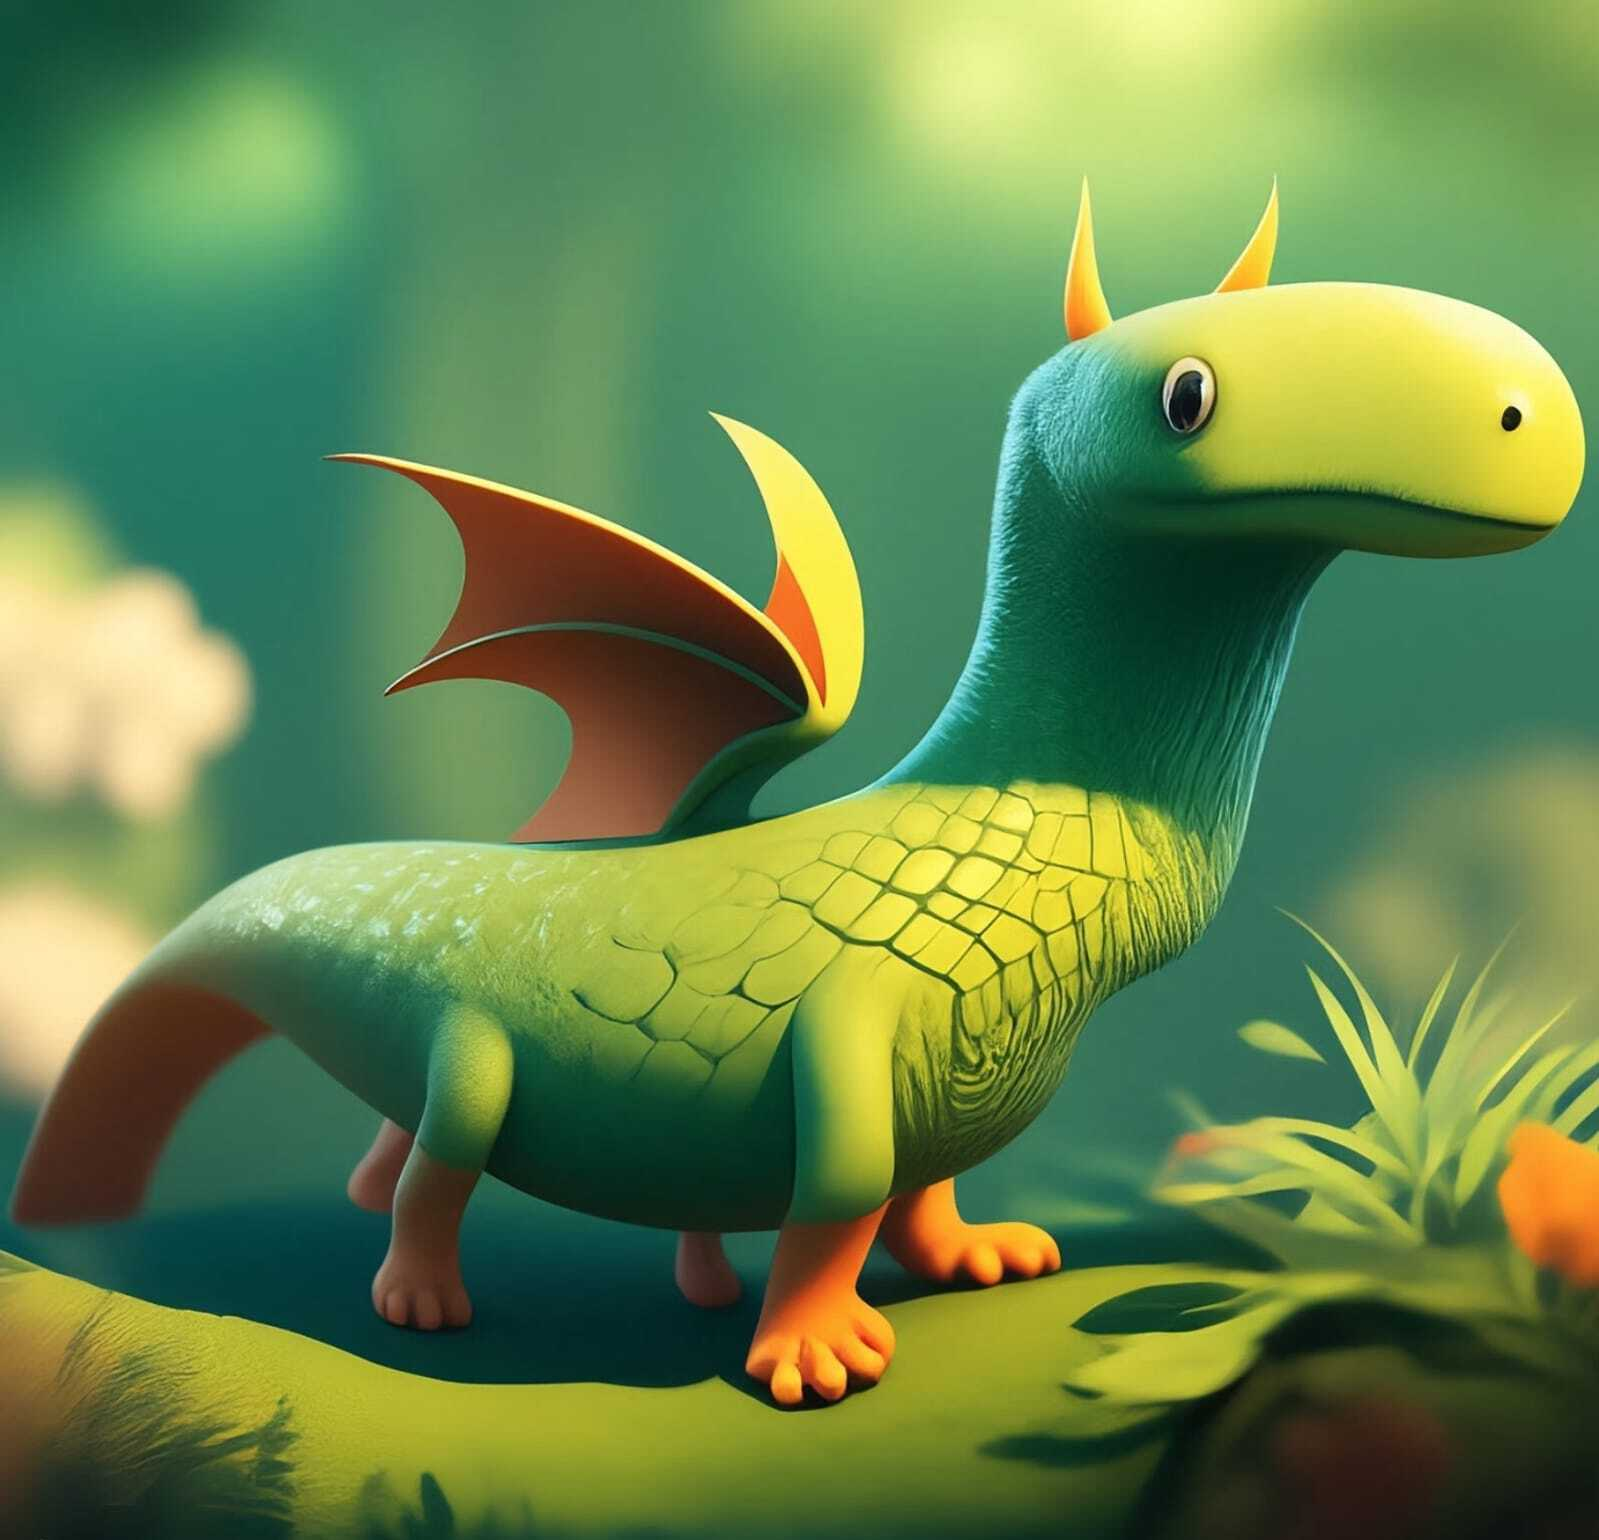
\includegraphics[width=6cm]{cover}
\end{center}
}

% theorem commands
\newtheoremstyle{c_remark}
	{}	% Space above
	{}	% Space below
	{}% Body font
	{}	% Indent amount
	{\bfseries}	% Theorem head font
	{}	% Punctuation after theorem head
	{.5em}	% Space after theorem head
	{\thmname{#1}\thmnumber{ #2}\thmnote{ \normalfont{\text{(#3)}}}}	% head content
\newtheoremstyle{c_definition}
	{3pt}	% Space above
	{3pt}	% Space below
	{}% Body font
	{}	% Indent amount
	{\bfseries}	% Theorem head font
	{}	% Punctuation after theorem head
	{.5em}	% Space after theorem head
	{\thmname{#1}\thmnumber{ #2}\thmnote{ \normalfont{\text{(#3)}}}}	% head content
\newtheoremstyle{c_plain}
	{3pt}	% Space above
	{3pt}	% Space below
	{\itshape}% Body font
	{}	% Indent amount
	{\bfseries}	% Theorem head font
	{}	% Punctuation after theorem head
	{.5em}	% Space after theorem head
	{\thmname{#1}\thmnumber{ #2}\thmnote{ \text{(#3)}}}	% head content

\ifcsname c@english\endcsname
	\theoremstyle{plain}
	\newtheorem{theorem}{Theorem}[section]
	\newtheorem{lemma}[theorem]{Lemma}
	\newtheorem{proposition}[theorem]{Proposition}
	\newtheorem*{proposition*}{Proposition}
	%\newtheorem{corollary}[theorem]{אין חלופה עברית}

	\theoremstyle{definition}
	\newtheorem{definition}[theorem]{Definition}
	\newtheorem*{definition*}{Definition}
	\newtheorem{example}{Example}[section]
	\newtheorem{exercise}{Exercise}[section]

	\theoremstyle{remark}
	\newtheorem*{remark}{Remark}
	\newtheorem*{solution}{Solution}
	\newtheorem{conclusion}[theorem]{Conclusion}
	\newtheorem{notation}[theorem]{Notation}
\else
	\theoremstyle{c_plain}
	\newtheorem{theorem}{משפט}[section]
	\newtheorem{lemma}[theorem]{למה}
	\newtheorem{proposition}[theorem]{טענה}
	\newtheorem*{proposition*}{טענה}
	%\newtheorem{corollary}[theorem]{אין חלופה עברית}

	\theoremstyle{c_definition}
	\newtheorem{definition}[theorem]{הגדרה}
	\newtheorem*{definition*}{הגדרה}
	\newtheorem{example}{דוגמה}[section]
	\newtheorem{exercise}{תרגיל}[section]

	\theoremstyle{c_remark}
	\newtheorem*{remark}{הערה}
	\newtheorem*{solution}{פתרון}
	\newtheorem{conclusion}[theorem]{מסקנה}
	\newtheorem{notation}[theorem]{סימון}
\fi

% Questions related commands
\newcounter{question}
\setcounter{question}{1}
\newcounter{sub_question}
\setcounter{sub_question}{1}

\ifcsname c@english\endcsname
	\newcommand{\question}[1][0]{
		\ifthenelse{#1 = 0}{}{\setcounter{question}{#1}}
		\section{Question \arabic{question}}
		\addtocounter{question}{1}
		\setcounter{sub_question}{1}
	}

	\newcommand{\subquestion}[1][0]{
		\ifthenelse{#1 = 0}{}{\setcounter{sub_question}{#1}}
		\subsection{Part \alph{sub_question}}
		\addtocounter{sub_question}{1}
	}
\else
	\newcommand{\question}[1][0]{
		\ifthenelse{#1 = 0}{}{\setcounter{question}{#1}}
		\section{שאלה \arabic{question}}
		\addtocounter{question}{1}
		\setcounter{sub_question}{1}
	}

	\newcommand{\subquestion}[1][0]{
		\ifthenelse{#1 = 0}{}{\setcounter{sub_question}{#1}}
		\subsection{סעיף \localecounter{letters.gershayim}{sub_question}}
		\addtocounter{sub_question}{1}
	}
\fi

% import lua and start of document
\directlua{common = require ('../common')}

\GetEnv{AUTHOR}

% headers
\author{\AUTHOR}
\date\today

\title{פתרון מטלה 04 --- פונקציות מרוכבות, 80519}

\begin{document}
\maketitle
\maketitleprint{}

\Question{}
תהי $U \subseteq \CC$ ונוכיח את הזהויות הבאות עבור $f, g \in C^1(U)$.

\Subquestion{}
\[
	\frac{\partial}{\partial z}(f \cdot g) = \frac{\partial f}{\partial z} \cdot g + f \cdot \frac{\partial g}{\partial z}
\]
\begin{proof}
	נבחן ישירות מהגדרת הגבול
	\begin{align*}
		\frac{\partial (f \cdot g)}{\partial z}
		& = \lim_{h \to 0} \frac{f(z + h) g(z + h) - f(z) g(z)}{h} \\
		& = \lim_{h \to 0} \frac{(f(z + h) - f(z)) g(z + h) + f(z) g(z + h) - f(z) g(z)}{h} \\
		& = \lim_{h \to 0} \frac{(f(z + h) - f(z)) g(z + h)}{h} + \lim_{h \to 0} \frac{f(z) g(z + h) - f(z) g(z)}{h} \\
		& = \lim_{h \to 0} g(z + h) \frac{f(z + h) - f(z)}{h} + \lim_{h \to 0} f(z) \frac{g(z + h) - g(z)}{h} \\
		& = \frac{\partial f}{\partial z} g + f \frac{\partial g}{\partial z}
	\end{align*}
\end{proof}

\Subquestion{}
\[
	\frac{\partial}{\partial z} (f \circ g)
	= \left( \frac{\partial f}{\partial z} \circ g \right) \frac{\partial g}{\partial z} + \left( \frac{\partial f}{\partial \overline{z}} \circ g \right) \frac{\partial \overline{g}}{\partial z}
\]
\begin{proof}
	נבצע חישובים חלקיים:
	\[
		\frac{\partial (f \circ g)}{\partial x}
		= \frac{\partial f(g, \overline{g})}{\partial x}
		= \left(\frac{\partial f}{\partial x} \circ g\right) \cdot \left(\frac{\partial g}{\partial x} + \frac{\partial \overline{g}}{\partial x}\right)
	\]
	וכן גם
	\[
		\frac{\partial (f \circ g)}{\partial y}
		= \left(\frac{\partial f}{\partial y} \circ g\right) \cdot \left(\frac{\partial g}{\partial y} - \frac{\partial \overline{g}}{\partial y}\right)
	\]
	ולבסוף אנו יודעים כי
	\[
		\frac{\partial (f \circ g)}{\partial z}
		= \frac{1}{2} \left(\frac{\partial f}{\partial x} - i \frac{\partial f}{\partial y}\right)
	\]
	ומהרכבת שלושת השוויונות האחרונים נקבל את השוויון המבוקש:
	\[
		\frac{\partial}{\partial z} (f \circ g)
		= \left( \frac{\partial f}{\partial z} \circ g \right) \frac{\partial g}{\partial z} + \left( \frac{\partial f}{\partial \overline{z}} \circ g \right) \frac{\partial \overline{g}}{\partial z}
	\]
\end{proof}

\Subquestion{}
\[
	\frac{\partial \overline{f}}{\partial \overline{z}}
	= \overline{\left( \frac{\partial f}{\partial z} \right)}
\]
\begin{proof}
	נשתמש באופרטור Wirtinger של $f$ ונגזור לפי $\overline{z}$:
	\begin{align*}
		\frac{\partial \overline{f}}{\partial \overline{z}}
		& = \frac{1}{2} (\frac{\partial \overline{f}}{\partial x} + i\frac{\partial \overline{f}}{\partial y}) \\
		& = \frac{1}{2} (\frac{\partial (u - i v)}{\partial x} + i\frac{\partial (u - i v)}{\partial y}) \\
		& = \frac{1}{2} (\frac{\partial u}{\partial x} - i \frac{\partial v}{\partial x} + i \frac{\partial u}{\partial y} + \frac{\partial v}{\partial y}) \\
		& = \frac{1}{2} \overline{(\frac{\partial u}{\partial x} + i \frac{\partial v}{\partial x} - i \frac{\partial u}{\partial y} + \frac{\partial v}{\partial y})} \\
		& = \frac{1}{2} \overline{(\frac{\partial (u + iv)}{\partial x} - i \frac{\partial (u + iv)}{\partial y})} \\
		& = \overline{\left(\frac{\partial f}{\partial z}\right)}
	\end{align*}
\end{proof}

\Question{}
נמצא את כל הנקודות בהן הפונקציות הנתונות גזירות.

\Subquestion{}
נגדיר $f(z) = \sin(\overline{z})$.
\begin{solution}
	נבחין כי כאופרטור Wirtinger מתקיים
	\[
		f(z, \overline{z})
		= \sin(\overline{z})
		= \frac{e^{i \overline{z}} - e^{-i \overline{z}}}{2i}
		= \frac{e^{i (x - iy)} - e^{-i (x - iy)}}{2i}
		= \frac{e^{ix + y} - e^{-ix - y}}{2i}
	\]
	ובתרגול ראינו כי הפונקציה גזירה אם ורק אם $\frac{\partial f}{\partial \overline{z}} = 0$, לכן נבדוק:
	\[
		\frac{\partial f}{\partial \overline{z}}
		= \frac{1}{2} (\frac{\partial f}{\partial x} + i \frac{\partial f}{\partial y})
		= \frac{1}{2} (\frac{1}{2i}(i e^{ix + y} + i e^{-ix - y} + i(e^{ix + y} + e^{-ix - y})))
		= \frac{1}{2}(e^{ix + y} + e^{-ix - y})
		= \cos(\overline{z})
	\]
	בדיעבד זה נובע ישירות. \\*
	נבדוק איפוס
	\[
		0 = \frac{\partial f}{\partial \overline{z}} = \cos(\overline{z})
	\]
	וממטלה 2 נסיק שאלו הן הנקודות $z = \frac{\pi}{2} + \pi k + 0 i$.
\end{solution}

\Subquestion{}
נגדיר $g(z) = e^{{|z - 1|}^2}$.
\begin{solution}
	נבחין כי מתקיים $e^{{|z - 1|}^2} = e^{(z - 1) \overline{(z - 1)}} = e^{z \overline{z} - z - \overline{z} + 1}$ ולכן
	\[
		g(z, \overline{z}) = \exp(z \overline{z} - z - \overline{z} + 1)
	\]
	ובהתאם
	\[
		\frac{\partial g}{\partial \overline{z}} = (z - 1) \exp(z \overline{z} - z - \overline{z} + 1)
	\]
	אז מתקיים
	\[
		\frac{\partial g}{\partial \overline{z}} = 0
		\iff (z - 1) g(z, \overline{z}) = 0
		\iff z = 1, g(z, \overline{z}) = 0
	\]
	אבל $g$ לא מתאפסת כאקספוננט ממשי, ולכן $g$ גזירה ב־$z = 1$ בלבד.
\end{solution}

\Subquestion{}
נגדיר $h(z) = \overline{\Log(z)} - {|z|}^2$.
\begin{solution}
	במקרה זה מתקיים
	\[
		h(z, \overline{z}) = \log(\sqrt{z \overline{z}}) - \Arg(z) - z \overline{z}
	\]
	ולכן
	\[
		\frac{\partial h}{\partial \overline{z}}
		= \frac{\frac{\sqrt{z}}{2 \sqrt{\overline{z}}}}{\sqrt{z \overline{z}}} - z
		= \frac{1}{2 \overline{z}} - z
	\]
	נשווה לאפס
	\[
		\frac{\partial h}{\partial \overline{z}} = 0
		\iff 1 = 2 z \overline{z}
		\iff |z| = \frac{1}{\sqrt{2}}
	\]
	ולכן הפונקציה גזירה על המעגל $\partial B(0, \frac{1}{\sqrt{2}})$.
\end{solution}

\Question{}
נגדיר
\[
	f(z) = \begin{cases}
		{\left(\frac{z}{|z|}\right)}^4 & z \ne 0 \\
		1 & z = 0
	\end{cases}
\]
ונוכיח כי $f$ דיפרנציאבילית כפונקציה ממשית ב־$\CC \setminus \{ 0 \}$, מקיימת את משוואות קושי־רימן ב־$z = 0$ ולמרות זאת אינה גזירה באף נקודה.
\begin{proof}
	כדי ש־$f$ תהיה דיפרנציאבילית בתחום הנתון, די לבדוק את הנגזרות החלקיות שלה בתחום:
	\begin{align*}
		& \frac{\partial f}{\partial x}
		= \frac{\partial}{\partial x} {\left(\frac{x + iy}{\sqrt{x^2 + y^2}}\right)}^4
		= \frac{\partial}{\partial x} {\left(\frac{{(x + iy)}^2}{x^2 + y^2}\right)}^2 \\
		= & 2 \left(\frac{{(x + iy)}^2}{x^2 + y^2}\right) \cdot \frac{(2x + 2iy)(x^2 + y^2) - 2x {(x + iy)}^2}{{(x^2 + y^2)}^2}
		= 4 \frac{{(x + iy)}^3}{{(x^2 + y^2)}^3} \cdot (y^2 - i x y)
	\end{align*}
	וכן באופן דומה גם
	\[
		\frac{\partial f}{\partial y}
		= 2 \left(\frac{{(x + iy)}^2}{x^2 + y^2}\right) \cdot \frac{(-2y + 2ix)(x^2 + y^2) - 2y {(x + iy)}^2}{{(x^2 + y^2)}^2}
		= 4 \frac{{(x + iy)}^3}{{(x^2 + y^2)}^3} \cdot (ix^2 - y x)
	\]
	מצאנו ביטוי רציף בתחום לשתי הפונקציות ולכן נסיק כי $f$ אכן דיפרנציאבילית.

	עוד נבחין כי הפונקציה כפונקציה ממשית היא רציפה ב־0 ונחשב את הנגזרות החלקיות שם בהתאם לביטויים שמצאנו:
	\[
		\frac{\partial f}{\partial z} \mid_0
		= \lim_{x \to 0} 4 \frac{x^3}{x^6} \cdot 0
		= 0
	\]
	ובאותו אופן נקבל גם $\frac{\partial f}{\partial y} \mid_0 = 0$ ולכן הפונקציה דיפרנציאבילית ב־$z = 0$ ומשוואות קושי־רימן מתקיימות (עבור 0). \\*
	לבסוף נבחין שממשוואות קושי־רימן עבור הנגזרות שמצאנו מתקבל שהפונקציה גזירה $y^2 = -yx$ וכן $-xy = yx$ וזה כמובן מתקיים רק ב־0, אך הפונקציה כלל לא רציפה בנקודה זו לפי בחירת סדרה מתאימה ושימוש באפיון היינה לגבולות.
\end{proof}

\Question{}
בכל סעיף נגדיר פונקציה ונוכיח שהיא הרמונית, ולאחר מכן נחשב את הצמוד ההרמוני שלה.

\Subquestion{}
נגדיר $u_1(x, y) = e^x (y \cos y + x \sin y)$.
\begin{proof}
	נחשב
	\[
		\nabla u_1 = (e^x (y \cos y + x \sin y + \sin y), e^x(\cos y - y \sin y + x \cos y))
	\]
	ולכן
	\[
		\frac{\partial^2 f}{\partial x^2} + \frac{\partial^2 f}{\partial y^2}
		= e^x (y \cos y + x \sin y + 2 \sin y) + e^x (-\sin y - \sin y - y \cos y - x \sin y)
		= e^x (0)
		= 0
	\]
	אז $u_1$ היא אכן פונקציה הרמונית, ונעבור לחישוב הצמוד ההרמוני שלה.
	נגדיר
	\begin{align*}
		v_1(x, y)
		& = C - \int_{0}^{x} \frac{\partial u_1}{\partial y}(t, 0)\ dt + \int_{0}^{y} \frac{\partial u_1}{\partial x}(0, t)\ dt \\
		& = C - \int_{0}^{x} e^t (1 - 0 + t)\ dt + \int_{0}^{y} e^0 (t \cos t + 0 + \sin t)\ dt \\
		& = C - x e^x + y \sin y
	\end{align*}
	ולכן $v_1(x, y) = y \sin y - x e^x$ המשלים ההרמוני של $u_1$.
\end{proof}

\Subquestion{}
נגדיר $u_2(x, y) = x^3 - 3 x y^2 + 6x y - 3x$.
\begin{proof}
	נגזור
	\[
		\nabla u_2 = (3x^2 - 3y^2 + 6y - 3, -6x y + 6x)
	\]
	ולכן
	\[
		\triangle u_2 = 6x - 6x = 0
	\]
	ואכן הפונקציה הרמונית, נעבור לחישוב המשלים
	\[
		v_2(x, y)
		= C - \int_{0}^{x} \frac{\partial u_2}{\partial y}(t, 0)\ dt + \int_{0}^{y} \frac{\partial u_2}{\partial x}(0, t)\ dt
		= C - 3x^2 - y^3 + 3y^2 - 3y
	\]
	ולכן הצמוד ההרמוני הוא $v_2(x, y) = -3x^2 - y^3 + 3y^2 - 3y$.
\end{proof}

\Subquestion{}
נגדיר $u_3(x, y) = \frac{x}{x^2 + y^2}$.
\begin{proof}
	הפעם
	\[
		\nabla u_3 = (\frac{y^2 - x^2}{{(x^2 + y^2)}^2}, \frac{-2xy}{{(x^2 + y^2)}^2})
	\]
	ולכן
	\[
		\triangle u_3 = \frac{-2x {(x^2 + y^2)}^2 - 2 (x^2 + y^2) 2x (y^2 - x^2) + -2x {(x^2 + y^2)}^2 - 2 (x^2 + y^2) 2y (-2xy)}{{(x^2 + y^2)}^4} = 0
	\]
	ולכן הפונקציה הרמונית ונשאר לחשב את המשלים ההרמוני שלה.
	\begin{align*}
		v_3(x, y)
		& = C - \int_{1}^{x} \frac{\partial u_3}{\partial y}(t, 0)\ dt + \int_{0}^{y} \frac{\partial u_3}{\partial x}(1, t)\ dt \\
		& = C - \int_{1}^{x} \frac{0}{{(t^2 + 0^2)}^2}\ dt + \int_{0}^{y} \frac{t^2 - 1^2}{{(1^2 + t^2)}^2}\ dt \\
		& = C + \arctan y - 2 \int_{0}^{y} \frac{1}{{(1 + t^2)}^2}\ dt \\
		& = C - \frac{y}{y^2 + 1}
	\end{align*}
	ולכן $v_3(x, y) = - \frac{y}{y^2 + 1}$.
\end{proof}

\Question{}
יהי $G \subseteq \CC$ תחום ו־$u, v : G \to \RR$ פונקציות הרמוניות כך ש־$v$ צמודה הרמונית של $u$.

\Subquestion{}
נוכיח כי אם $w$ צמודה הרמונית נוספת של $u$ אז $v - w$ בהכרח קבועה.
\begin{proof}
	נבחין כי הן $u + i v$ והן $u + i w$ פונקציות אנליטיות ולכן מתקיים מקושי־רימן
	\[
		\frac{\partial u}{\partial x} = \frac{\partial v}{\partial y},
		\frac{\partial u}{\partial y} = -\frac{\partial v}{\partial x}
	\]
	אבל גם
	\[
		\frac{\partial u}{\partial x} = \frac{\partial w}{\partial y},
		\frac{\partial u}{\partial y} = -\frac{\partial w}{\partial x}
	\]
	ולכן נובע ישירות
	\[
		\frac{\partial v}{\partial x} = \frac{\partial w}{\partial x},
		\frac{\partial v}{\partial y} = \frac{\partial w}{\partial y}
	\]
	ולכן $v$ ו־$w$ זהות עד כדי קבוע, דהינו $v - w$ פונקציה קבועה.
\end{proof}

\Subquestion{}
נוכיח כי אם $u$ גם צמודה הרמונית של $v$ אז $u, v$ בהכרח קבועות.
\begin{proof}
	נתון כי $u + iv$ אנליטית וכן $v + iu$ אנליטית, לכן מתקיים
	\[
		\frac{\partial u}{\partial x} = \frac{\partial v}{\partial y},
		\frac{\partial u}{\partial y} = -\frac{\partial v}{\partial x}
	\]
	אבל גם
	\[
		\frac{\partial v}{\partial x} = \frac{\partial u}{\partial y},
		\frac{\partial v}{\partial y} = -\frac{\partial u}{\partial x}
	\]
	ולכן נובע
	\[
		\frac{\partial u}{\partial x} = -\frac{\partial u}{\partial x}
	\]
	ונובע $\frac{\partial u}{\partial x} = 0$ ובאותו אופן נקבל את איפוס כל שאר הנגזרות החלקיות, ולכן $u, v$ פונקציות קבועות.
\end{proof}

\Subquestion{}
נוכיח כי אם $u^2 + v^2 = 1$ אז $u, v$ בהכרח קבועות.
\begin{proof}
	מהנתון נובע
	\[
		\frac{\partial}{\partial x} (u^2 + v^2) = 0
		\iff \frac{\partial u}{\partial x} = -\frac{\partial v}{\partial x}
	\]
	ובאופן דומה
	\[
		\frac{\partial u}{\partial y} = -\frac{\partial v}{\partial y}
	\]
	ובשילוב זהה לסעיף הקודם עם משוואות קושי־רימן נובע כי $u, v$ קבועות.
\end{proof}

\Subquestion{}
נוכיח כי $u^2 - v^2$ ו־$uv$ הרמוניות.
\begin{proof}
	נחשב את הלפלסיאן של הפונקציות החדשות:
	\begin{align*}
		\triangle (u^2 - v^2)
		& = \frac{\partial^2}{\partial x^2}(u^2 - v^2) + \frac{\partial^2}{\partial y^2}(u^2 - v^2) \\
		& = \frac{\partial}{\partial x}(2u \frac{\partial u}{\partial x} - 2v \frac{\partial v}{\partial x}) + \frac{\partial}{\partial y}(2u \frac{\partial u}{\partial y} - 2v \frac{\partial v}{\partial y}) \\
		& = 2\frac{\partial^2 u}{\partial x^2} + 2 {\left(\frac{\partial u}{\partial x}\right)}^2 - 2\frac{\partial^2 v}{\partial x^2} - 2 {\left( \frac{\partial v}{\partial x}\right)}^2
		+ 2\frac{\partial^2 u}{\partial y^2} + 2 {\left(\frac{\partial u}{\partial y}\right)}^2 - 2\frac{\partial^2 v}{\partial y^2} - 2 {\left( \frac{\partial v}{\partial y}\right)}^2 \\
		& = 0
	\end{align*}
	כאשר המעבר האחרון היה שימוש בלפלסיאנים של $u, v$.

	באופן דומה נבחן את הלפלסיאן של $u v$:
	\begin{align*}
		\triangle u v
		& = \frac{\partial^2}{\partial x^2} u v + \frac{\partial^2}{\partial y^2} u v \\
		& = \frac{\partial}{\partial x} (\frac{\partial u}{\partial x} v + \frac{\partial v}{\partial x} u) + \frac{\partial}{\partial y} (\frac{\partial u}{\partial y} v + \frac{\partial v}{\partial y} u) \\
		& = \frac{\partial^2 u}{\partial x^2} v + 2 \frac{\partial u}{\partial x} \cdot \frac{\partial v}{\partial x} + \frac{\partial^2 v}{\partial x^2} u +
		\frac{\partial^2 u}{\partial y^2} v + 2 \frac{\partial u}{\partial y} \cdot \frac{\partial v}{\partial y} + \frac{\partial^2 v}{\partial y^2} u \\
		& = 2 \frac{\partial u}{\partial x} \cdot \frac{\partial v}{\partial x} + 2 \frac{\partial u}{\partial y} \cdot \frac{\partial v}{\partial y} \\
		& \overset{C.S.}{=} 2 \frac{\partial u}{\partial x} \cdot \frac{\partial v}{\partial x} - 2 \frac{\partial v}{\partial x} \cdot \frac{\partial u}{\partial x} \\
		& = 0
	\end{align*}
\end{proof}

\Question{}
יהי $G \subseteq \CC$ כדור פתוח ו־$h \in C^2(G)$.
נוכיח כי $h(z) = f(z) + \overline{g(z)}$ עבור פונקציות אנליטיות $f, g : G \to \CC$ אם ורק אם $h = u + i v$ עבור $u, v : G \to \RR$ הרמוניות.
\begin{proof}
	נניח ש־$h = f + \overline{g}$ עבור $f, g$ אנליטיות בתחום. \\*
	לכן מטענה מהכיתה נובע $f = u + i \tilde{u}$ ו־$g = v + i \tilde{v}$ עבור $u, v \in Harm(G)$. \\*
	בהתאם נובע ש־$h = (u + v) + i (\tilde{u} - \tilde{v})$, אבל גם $u + v, \tilde{u} - \tilde{v} \in Harm(G)$ וקיבלנו את הרצוי.

	נניח ש־$h = u + i v$ עבור $u, v \in Harm(G)$. \\*
	נגדיר $f = u_f + i v_f, g = u_g + i v_g$ כך שמתקיים
	\[
		h = u + i v = f + \overline{g} = (u_f + u_g) + i (v_f - v_g)
	\]
	ולכן
	\[
		u = u_f + u_g,
		\qquad
		v = v_f - v_g
	\]
	נגזור את הביטויים ונשתמש בקושי־רימן:
	\begin{align*}
		& \frac{\partial u}{\partial x} && = \frac{\partial u_f}{\partial x} + \frac{\partial u_g}{\partial x} && = \frac{\partial v_f}{\partial y} + \frac{\partial v_g}{\partial y} \\
		& \frac{\partial u}{\partial y} && = \frac{\partial u_f}{\partial y} + \frac{\partial u_g}{\partial y} && = -\frac{\partial v_f}{\partial y} - \frac{\partial v_g}{\partial y} \\
		& \frac{\partial v}{\partial x} && = \frac{\partial v_f}{\partial x} + \frac{\partial v_g}{\partial x} && = -\frac{\partial u_f}{\partial y} + \frac{\partial u_g}{\partial y} \\
		& \frac{\partial v}{\partial y} && = \frac{\partial v_f}{\partial y} + \frac{\partial v_g}{\partial y} && = \frac{\partial u_f}{\partial x} - \frac{\partial u_g}{\partial x} \\
	\end{align*}
	לכן נוכל להסיק ש־$\frac{\partial u_f}{\partial x} = \frac{1}{2} (\frac{\partial u}{\partial x} + \frac{\partial v}{\partial y})$, ועל־ידי אינטגרציה נמצא ביטוי ל־$u_f$. \\*
	נחזור על תהליך זה ונקבל $f, g$ כמבוקש.
\end{proof}

\end{document}
